\section{System Architecture}
\label{sec:req-architecture}

Figure~\ref{fig:req-hardware-architecture} shows the power path from the mains to the connector and the feedback path to the controller. Input protection, filtering, and rectification feed the charge-pump branch and DC link. The shared GaN half bridge then drives both input charge transfer and isolated resonant transfer.



The transformer transfers power across the isolation barrier. The secondary rectifier and capacitor supply the bulk node, from which the MPQ4242 section supplies VBUS. The AMC0330 returns bulk-voltage feedback to the primary-referenced MCU across a separate sensing barrier.

On the original prototype, MCU pins PA8 and PA9 generate complementary carrier commands, while PA10 enables switching bursts. Primary-voltage (PA0), secondary-voltage (PA1), and half-bridge-current (PA2) signals are acquired by a continuous ADC scan and buffered by DMA. Sampling is asynchronous to the carrier.

Auxiliary rails supply the gate drive, MCU, sensing, and output interface. These rails must be checked with the carrier inhibited before feedback calibration and low-power transfer. Closed-loop regulation requires valid isolated feedback.

The resonant paths meet at the switch node. Burst control consequently changes both secondary transfer and the mains-current envelope; the next chapter analyzes this coupling.

\begin{figure}[H]
\centering
\begingroup
\definecolor{reqNavy}{HTML}{153448}
\definecolor{reqTeal}{HTML}{007C83}
\definecolor{reqRed}{HTML}{990000}
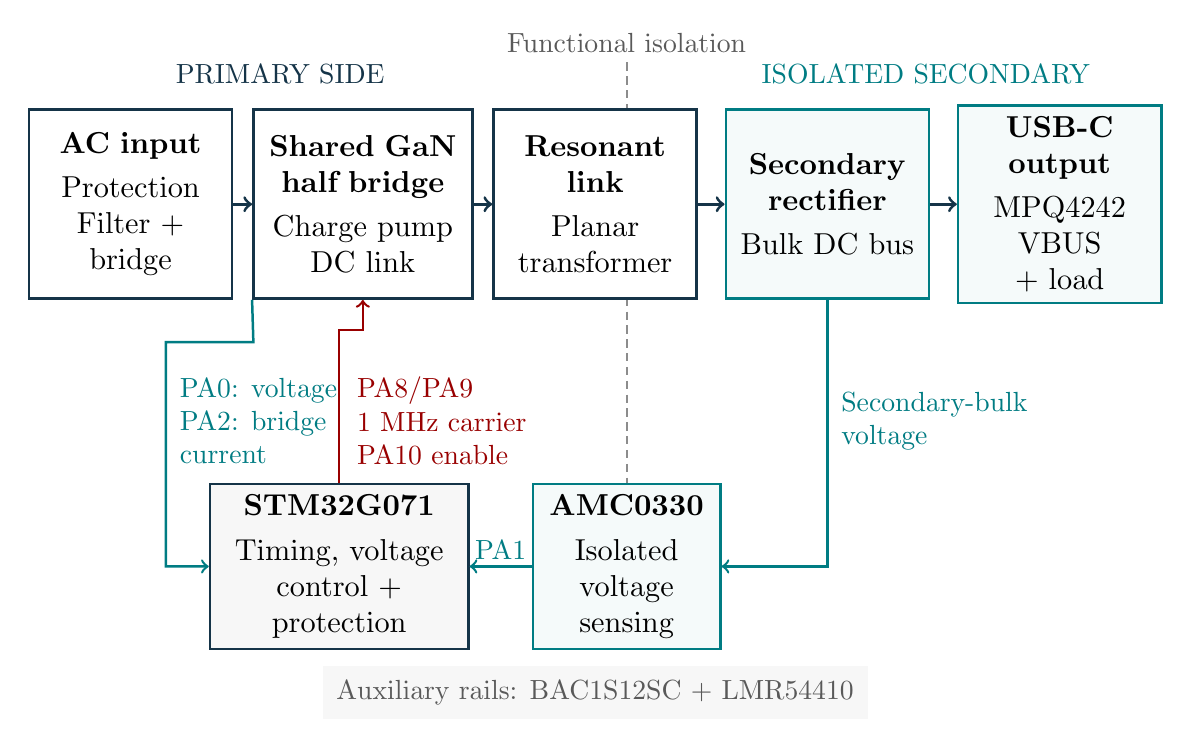
\begin{tikzpicture}[
    font=\fontsize{11}{13}\selectfont,
    block/.style={
        draw=reqNavy,fill=white,line width=0.9pt,
        text width=2.3cm,minimum height=2.4cm,
        align=center,inner sep=4pt,
        execute at begin node={\hyphenpenalty=10000\exhyphenpenalty=10000}
    },
    secondary/.style={block,draw=reqTeal,fill=reqTeal!4},
    controller/.style={
        block,text width=3.0cm,minimum height=1.5cm,fill=black!3
    },
    sensor/.style={
        block,draw=reqTeal,text width=2.1cm,
        minimum height=1.5cm,fill=reqTeal!4
    },
    powerflow/.style={->,draw=reqNavy,line width=1.1pt},
    feedback/.style={->,draw=reqTeal,line width=0.9pt},
    command/.style={->,draw=reqRed,line width=0.9pt},
    signaltext/.style={
        font=\fontsize{10}{12}\selectfont,
        text=reqTeal,fill=white,inner sep=2pt,align=left
    }
]
% Draw the functional boundary first so the transformer and isolated
% sensing blocks visibly span it rather than implying a bare-wire crossing.
\draw[densely dashed,draw=black!45,line width=0.8pt]
    (6.3,1.8) -- (6.3,-5.55);
\node[font=\fontsize{10}{12}\selectfont,text=reqNavy]
    at (1.9,1.65) {PRIMARY SIDE};
\node[font=\fontsize{10}{12}\selectfont,text=reqTeal]
    at (10.1,1.65) {ISOLATED SECONDARY};
\node[font=\fontsize{10}{12}\selectfont,text=black!65,
    fill=white,inner sep=2pt]
    at (6.3,2.05) {Functional isolation};

\node[block] (front) at (0,0)
    {\textbf{AC input}\\[3pt]Protection\\Filter + bridge};
\node[block,text width=2.5cm] (shared) at (2.95,0)
    {\textbf{Shared GaN}\\\textbf{half bridge}\\[3pt]Charge pump\\DC link};
\node[block] (link) at (5.9,0)
    {\textbf{Resonant}\\\textbf{link}\\[3pt]Planar\\transformer};
\node[secondary] (bulk) at (8.85,0)
    {\textbf{Secondary}\\\textbf{rectifier}\\[3pt]Bulk DC bus};
\node[secondary] (output) at (11.8,0)
    {\textbf{USB-C}\\\textbf{output}\\[3pt]MPQ4242\\VBUS + load};

\draw[powerflow] (front.east) -- (shared.west);
\draw[powerflow] (shared.east) -- (link.west);
\draw[powerflow] (link.east) -- (bulk.west);
\draw[powerflow] (bulk.east) -- (output.west);

\node[controller] (mcu) at (2.65,-4.6)
    {\textbf{STM32G071}\\[3pt]Timing, voltage\\control + protection};
\node[sensor] (sense) at (6.3,-4.6)
    {\textbf{AMC0330}\\[3pt]Isolated\\voltage sensing};

% Keep the primary-side acquisition route separate from carrier/enable
% commands and the isolated secondary-voltage feedback route.
\draw[feedback] (shared.south west)
    -- (1.56,-1.75) -- (0.45,-1.75)
    -- (0.45,-4.6) -- (mcu.west);
\node[signaltext,anchor=west] at (0.55,-2.75)
    {PA0: voltage\\PA2: bridge\\current};

\draw[command] (mcu.north)
    -- (2.65,-1.6) -- (2.95,-1.6) -- (shared.south);
\node[signaltext,text=reqRed,anchor=west] at (2.8,-2.75)
    {PA8/PA9\\1 MHz carrier\\PA10 enable};

\draw[feedback] (bulk.south) -- (8.85,-4.6) -- (sense.east);
\node[signaltext,anchor=west] at (8.95,-2.75)
    {Secondary-bulk\\voltage};
\draw[feedback] (sense.west) -- node[
    above,font=\fontsize{10}{12}\selectfont,
    text=reqTeal,inner sep=2pt] {PA1} (mcu.east);

\node[font=\fontsize{10}{12}\selectfont,text=black!65,
    fill=black!3,inner sep=5pt]
    at (5.9,-6.2) {Auxiliary rails: BAC1S12SC + LMR54410};
\end{tikzpicture}
\endgroup
\caption{Power and control architecture of the V1.0 prototype with the V1.1 circuit corrections. The transformer carries power across the isolation barrier, and the AMC0330 returns secondary-bulk feedback to the MCU. PA1 measures this feedback; PA0 and PA2 measure primary voltage and half-bridge current.}
\label{fig:req-hardware-architecture}
\end{figure}
